\section{1. Summary}\label{sec:summary}

This system watches an office building for fire and acts on what it finds without
waiting for a person. Emulated smoke, carbon monoxide and temperature detectors
observe the true state of each room imperfectly; a detector turns their readings into
a probability of fire per room, and there are two of them to choose from, a
hand-written fusion rule and a language model asked over the network; a per-room
state machine climbs from
\textsc{normal} through \textsc{investigating} and \textsc{pre-alarm} to
\textsc{confirmed}; and on confirmation the system releases the sprinkler, closes the
fire door and sends the building out along routes that avoid the alarming rooms. The
building, its rooms and its 3D view are BuildSim's. This project supplies the fire
physics, the sensors, the intelligence and the response around it.

One principle runs through every decision below: \textbf{nothing downstream of the
sensors is allowed to see the truth}. The physics knows the real temperature of every
room. The detector, the agent and the interlocks only ever see what the sensors
reported. The gap between those two views is what the whole project studies, and the
dashboard shows the two side by side so that a false alarm or a missed fire is visible
as a mismatch rather than hidden in a log.

\begin{longtable}[]{@{}
  >{\raggedright\arraybackslash}p{(\columnwidth - 2\tabcolsep) * \real{0.28}}
  >{\raggedright\arraybackslash}p{(\columnwidth - 2\tabcolsep) * \real{0.72}}@{}}
\toprule
\textbf{Field} & \textbf{Value} \\
\midrule
\endhead
\textbf{Project title} & Fire Detection and Autonomous Response \\
\textbf{Team} & Group 14, Ekpenyong Esu Ekpenyong \\
\textbf{Use case} & Multi-modal fire detection with a verified alarm, interlocked
  suppression and containment, and evacuation routing on a three-storey building \\
\textbf{Repository} & \url{https://github.com/Ekpenyong-Esu/BuildSim-FireDetection} \\
\textbf{Version / date} & v10.1 / 2026-10-08 \\
\bottomrule
\end{longtable}

\textbf{Changes since the proposal.} Three things changed, each because building
the system taught something the proposal did not know.

\begin{itemize}[leftmargin=1.4em, itemsep=2pt]
\item \textbf{One process instead of a dozen.} The proposal sketched nine services
  joined by MQTT, with ThingsBoard for storage and dashboards. Its own risk list said
  the hardest part would be keeping a dozen processes synchronised in simulated time.
  That risk turned out to be the whole problem: at forty times real time a reading
  published over a broker is stale before the subscriber sees it, and the physics,
  the sensors and the agent must agree on what ``now'' is for a dwell time to mean
  anything. I therefore built the system as one tick loop with four zones inside
  it, and the separation the proposal wanted from process boundaries is enforced
  instead by import rules that a test checks (Section~\ref{sec:container}). The trade-off is
  discussed in Section~\ref{sec:risks}.
\item \textbf{The second detector is a language model, not an isolation forest.}
  The proposal planned to compare a hand-written fusion rule with a trained
  anomaly detector. The rule alone caught every real fire and raised no false alarm
  at any noise level tested (Section~\ref{sec:evaluation}), and the only data to train a forest on
  would have been the simulator's own output, so the comparison the proposal
  promised was made with a different second opinion: a language model behind an
  OpenAI-compatible endpoint, given the same readings the rule sees and nothing
  else, and asked for a probability, its evidence and a reason. It implements the
  same two-method protocol, so the agent, the interlocks and the dashboard did not
  change. Section~\ref{sec:service} says how it is kept off the tick and Section~\ref{sec:evaluation} reports the
  comparison. The short version: the model catches what the rule catches, later,
  at a fraction of the speed, and without repeatability; the rule remains the
  default.
\item \textbf{Containment against evacuation became an interlock, not a policy.}
  The proposal expected to tune a trade-off. In practice the safe rule is simple and
  should not be tunable: a fire door may not close on a room that is occupied or that
  lies on somebody's escape route, and doors never lock. The agent asks; the interlock
  decides; the request stands until it is safe to honour.
\end{itemize}

\section{2. Use case and building context (BuildSim)}\label{sec:usecase}

\textbf{The building.} The system runs on the A-building at Luleå University of
Technology as BuildSim models it: three storeys, 956 named spaces, 1005 doorways and
32 stairwells, and seven real exits, all on the ground floor. BuildSim owns the
floor plans, the walkable graph that joins rooms through their doors and the
stairwells that join the storeys, an equipment tree into which devices are
registered, and a 3D viewer fed over WebSocket. BuildSim is not modified. It is
instrumented and drawn on.

\textbf{What BuildSim does not provide} is anything that changes over time: there
is no fire, no smoke, no people and no sensor physics. All of that is this project.
firelab loads the floor plans once, turns them into a graph of rooms and door-gated
couplings, and from then on writes back to BuildSim about once a simulated second:
floor heat maps of the true temperature, smoke and CO, particle effects for fire,
smoke and running sprinklers, the agent's alarm markers, fire-door state, every
occupant's position, and each device's latest reading into the equipment tree. Two
things are drawn into the viewer session rather than the building, because BuildSim
keeps them per browser tab: the coloured outlines of alarming rooms and the escape
route.

\textbf{Actors.} The \textbf{operator} watches the control panel, chooses what to
set on fire, injects sensor faults, picks which detector scores the rooms, and can
flip the system into supervised mode, where the agent still decides but a person
has to press the button. The
\textbf{occupants} are simulated people who influence nothing until the alarm sends
them walking, and whose presence in a room is what stops its door being closed.
Neither is on the control path. The loop from reading to sprinkler runs on its own.

\textbf{The scenario the demo tells.} A fast flaming fire starts in office A3505
on the top floor. Fifty-one seconds later the smoke reading has risen enough for the
room to start \textsc{investigating}; at 81\,s it is in \textsc{pre-alarm}, and at
106\,s, once the probability of fire has held above 0.75 for the confirmation dwell,
the room \textsc{confirms}. In the same tick the sprinkler is released because the
temperature reading corroborates the smoke, the fire door closes because the room
is empty and on nobody's route, and all 130 people in the building start walking to
a ground-floor exit along routes that avoid the alarming rooms. The last person is
out 111\,s after the alarm. Meanwhile the kitchen-cooking preset in the same room
produces smoke and warmth for fifteen minutes and never gets past
\textsc{investigating}, because its CO never rises.

\textbf{Why it matters.} A smoke detector cannot tell a fire from burnt toast, a
dusty corridor or its own drifting element. Real buildings are evacuated for all
three, and the cost of that is that alarms get ignored. Telling them apart needs
several modalities fused over time and across neighbouring rooms, which is a
genuine job for an autonomous service. The response has a real conflict inside it
too: closing a fire door holds the smoke back but takes away an escape route.
Latency, robustness to broken sensors, and the safety of the actions drive the
requirements that follow.

\textbf{Where it sits.} Fire detection is one of several systems that could run
on the same building: ventilation, security and energy management are the others in
the course. Each instruments BuildSim through the same API and each would be
watched by the same facilities staff. Figure~\ref{fig:landscape} shows the
landscape; this document designs the highlighted system. One thing in it reaches
off the laptop: when the language model is the chosen detector, the service asks
a chat endpoint over HTTPS about one room at a time. It is optional. Without it,
or when it is slow, the rule scores every room.

\begin{figure}[H]
\centering
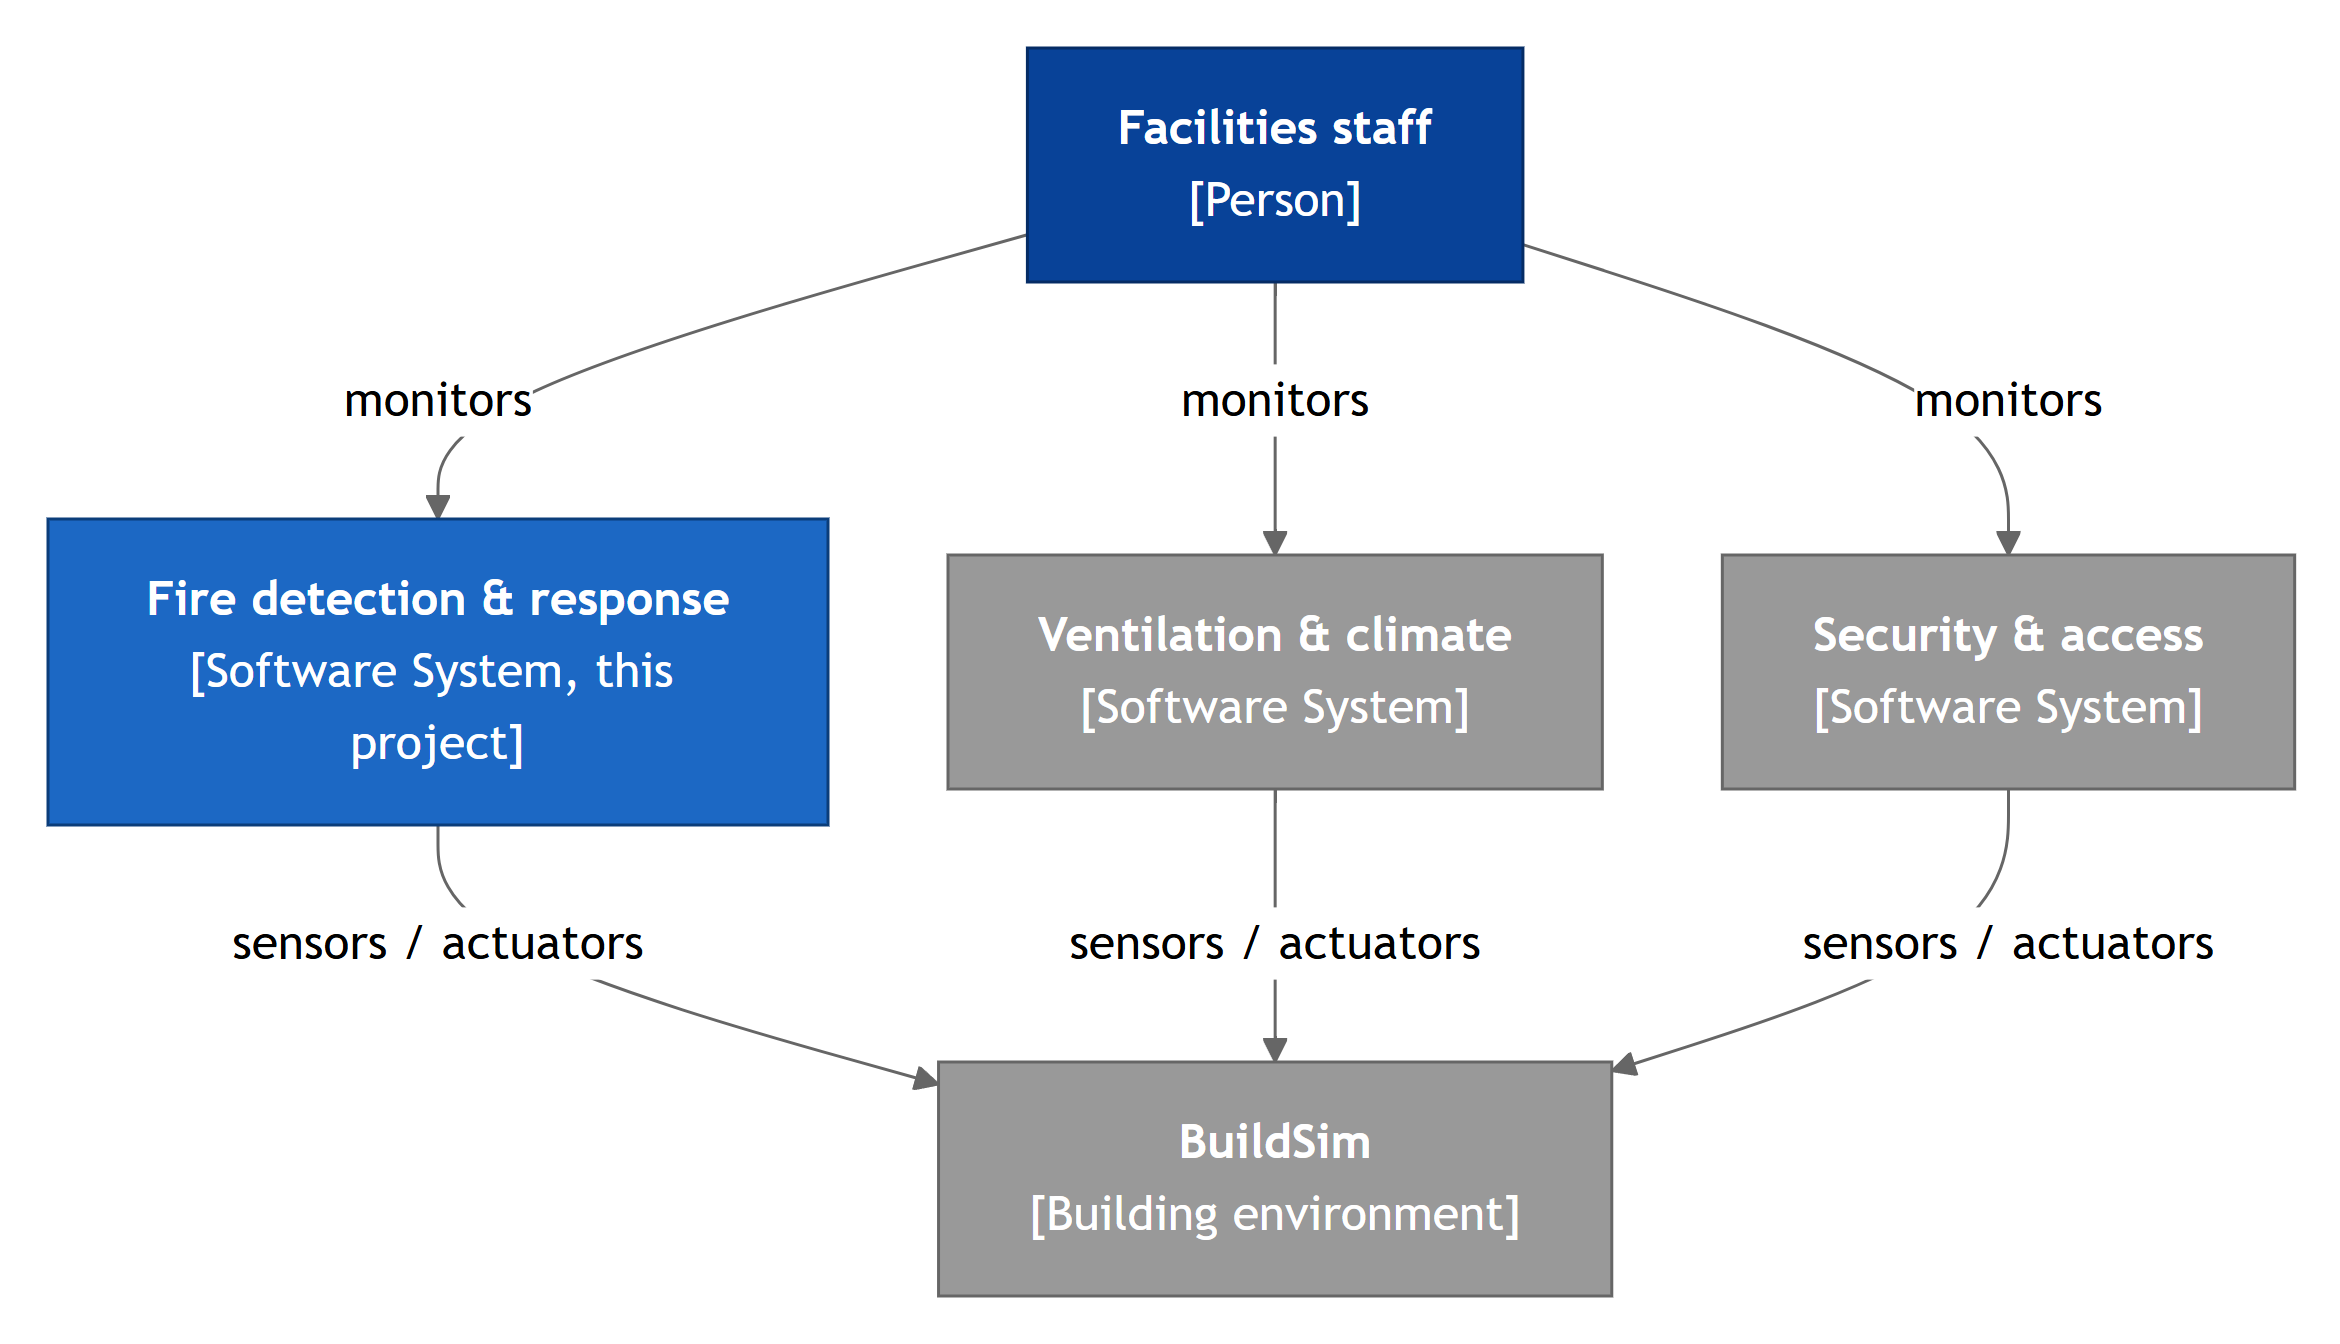
\includegraphics[width=0.85\linewidth]{images/landscape.png}
\caption{C4 System Landscape. Several building systems share one BuildSim; the highlighted one is designed here.}
\label{fig:landscape}
\end{figure}

\section{3. Requirements}\label{sec:requirements}

Every requirement is a testable statement with a stable ID. Functional requirements
(FR) say what the system does, safety requirements (SR) say what it must never do
whatever the agent decides, and non-functional requirements (NFR) say how well. The
last column names the test or experiment that verifies it; the test plan in
Section~10 and the results in Section~11 close the loop.

\begin{longtable}[]{@{}
  >{\raggedright\arraybackslash}p{(\columnwidth - 8\tabcolsep) * \real{0.08}}
  >{\raggedright\arraybackslash}p{(\columnwidth - 8\tabcolsep) * \real{0.28}}
  >{\raggedright\arraybackslash}p{(\columnwidth - 8\tabcolsep) * \real{0.08}}
  >{\raggedright\arraybackslash}p{(\columnwidth - 8\tabcolsep) * \real{0.30}}
  >{\raggedright\arraybackslash}p{(\columnwidth - 8\tabcolsep) * \real{0.26}}@{}}
\toprule
\textbf{ID} & \textbf{Requirement} & \textbf{Priority} & \textbf{Acceptance criterion} & \textbf{Verified by} \\
\midrule
\endhead
FR-01 & Confirm a flaming fire from sensor readings alone & Must & Room reaches \textsc{confirmed} within 180\,s of ignition & \code{test\_agent}, \code{test\_detector}, E1 \\
FR-02 & Confirm a smouldering fire, which has almost no heat & Must & \textsc{confirmed} within 300\,s (the scoreboard's miss limit) & E1 \\
FR-03 & Raise no alarm for cooking, dust, steam, or a drifting sensor & Must & Zero false alarms across all nuisance presets at sensor noise 0--3$\times$ & \code{test\_scoring}, E1, E3 \\
FR-04 & On confirmation: release sprinkler, close the fire door, evacuate & Must & All three commands issued in the confirming tick and journalled with a reason & \code{test\_agent}, E1 \\
FR-05 & Route every evacuee to a real ground-floor exit avoiding alarming rooms & Must & No route crosses an alarming room while a clear one exists; upper floors go down the stairs & \code{test\_evacuation}, \code{test\_walkways}, \code{test\_multifloor} \\
FR-06 & Explain every decision & Must & P(fire) is the sum of named contributions, or the model's verdict with its evidence and a one-line reason; every command and every refusal carries a reason & \code{test\_detector}, \code{test\_llm\_detector}, dashboard \\
FR-07 & Score the run against ground truth & Should & Detections, misses, false alarms, alarm delay and RSET reported live and exportable as CSV & \code{test\_scoring}, \code{test\_history} \\
FR-08 & A second detector behind the same protocol, switchable while running & Should & The language model scores rooms from readings only; the agent, interlocks and panel are unchanged; the panel can switch back & \code{test\_llm\_detector}, \code{test\_layering}, E7 \\
SR-01 & Water needs heat corroboration & Must & A sprinkler request is refused while the room's true temperature is below 35\,°C & \code{test\_interlocks}, E1 \\
SR-02 & Fire doors never lock & Must & A lock command is refused unconditionally & \code{test\_interlocks} \\
SR-03 & Never seal people in & Must & A close command is refused while the room is occupied or on an active escape route & \code{test\_interlocks}, \code{test\_publisher\_doors} \\
NFR-01 & Keep up with the clock & Must & One engine tick over the full building finishes inside the 250\,ms tick budget at 1$\times$; the breaking point at 40$\times$ is measured & E5 \\
NFR-02 & Survive a lying sensor & Must & A stuck, dropping-out or drifting smoke detector does not stop a flaming fire being confirmed & \code{test\_sensing}, E4 \\
NFR-03 & Be repeatable & Must & The same seed gives the same run, tick for tick & \code{test\_reset}, E1 (rerun) \\
NFR-04 & Keep the truth out of the intelligence & Must & No module downstream of the sensors imports or reads the true room state & \code{test\_layering} \\
NFR-05 & Not flood BuildSim & Should & At most 24 sensor writes per publish; the viewer route and highlights are sent only when they change & \code{test\_publishing\_route} \\
NFR-06 & Never wait for the model & Must & A tick never blocks on the network; a room with no fresh verdict is scored by the rule; a malformed answer is refused, not guessed at & \code{test\_llm\_detector} \\
NFR-07 & Never outrun the model & Must & A verdict older than 60 simulated seconds is not used; the speed dial is capped at what measured answer times allow, and the journal says so & \code{test\_pacing}, \code{test\_llm\_detector}, E7 \\
\bottomrule
\end{longtable}

There is a tension in this table. FR-01 and FR-02 want the alarm early;
FR-03 wants it late enough to be sure; SR-01 to SR-03 may refuse the response the
alarm asks for. The dwell times in the state machine resolve the first tension and
the interlocks resolve the second, and the evaluation reports where each of those
compromises costs something. NFR-06 and NFR-07 pull against each other too: a
detector that answers eight seconds late is useless at forty times real time, so
either the clock slows down or the rule takes over, and the system does the first
and falls back to the second. The safety requirements apply whichever detector is
installed; that is the point of keeping the interlocks outside the intelligence.

\textbf{Traceability.} The five architecture viewpoints map onto this document:
context (Section~4.1), functional (4.2 and 4.3), information (Sections~5 to~7),
behavioural (Section~8) and deployment (Section~9). Each requirement names the
design that satisfies it and the test that proves it.
